\documentclass[12pt]{kiarticle}
\graphicspath{{pictures/}}
\DeclareGraphicsExtensions{.pdf,.png,.jpg,.eps}
%%%
\pagestyle{fancy}
\fancyhf{}
%\renewcommand{\headrulewidth}{ 0.1mm }
\renewcommand{\footrulewidth}{ .0em }
\fancyfoot[C]{\texttt{\textemdash~\thepage~\textemdash}}
\fancyhead[L]{Лабораторная работа № \hfil}
\fancyhead[R]{\hfil Иванов Кирилл, 625 группа }
\usepackage{multirow} % Слияние строк в таблице
\newcommand
{\un}[1]
{\ensuremath{\text{#1}}}
\newcommand{\eds}{\ensuremath{ \mathscr{E}}}
\newcommand{\ga}{\ensuremath{\gamma}}
\usepackage{tikz}
%%% Работа с таблицами
\usepackage{array,tabularx,tabulary,booktabs} % Дополнительная работа с таблицами
\usepackage{longtable}  % Длинные таблицы
\usepackage{multirow} % Слияние строк в таблице

\begin{document}
	
	\begin{titlepage}
		\begin{center}
			\large 	Московский физико-технический институт \\
			(государственный университет) \\
			Факультет общей и прикладной физики \\
			\vspace{0.2cm}
			
			\vspace{4.5cm}
			Лабораторная работа №4.1  \\ \vspace{0.2cm}
			\large (Общая физика: квантовая физика) \\ \vspace{0.2cm}
			\LARGE \textbf{   }
		\end{center}
		\vspace{2.3cm} \large
		
		\begin{center}
			Работу выполнил: \\
			Иванов Кирилл,
			625 группа
			\vspace{10mm}		
			
		\end{center}
		
		\begin{center} \vspace{60mm}
			г. Долгопрудный \\
			2018 год
		\end{center}
	\end{titlepage}


	\paragraph*{Цель работы:} Измерить пробег альфа-частиц в воздухе двумя способами: с помощью торцевого счетчика Гейгера и ионизационной камеры. 
	
	
	\section{Теоретическое введение и описание установки}
	
	В качестве источника альфа-частиц используется $ ^{239}  $Pu  с периодом полураспада $ T_{1/2} = 2,44 \x 10^4 $ лет. Альфа-частицы, испускаемые $ ^{239} Pu $, состоят из трех моноэнергетических групп, различие между которы-
	ми лежит в пределах 50 кэВ. При той точности, которая достигается
	в наших опытах, их можно считать совпадающими по энергии, равной
	5,15 МэВ.
	
	\subsection{Счетчик Гейгера}
	
	\begin{wrapfigure}[15]{l}{0.25\linewidth}
		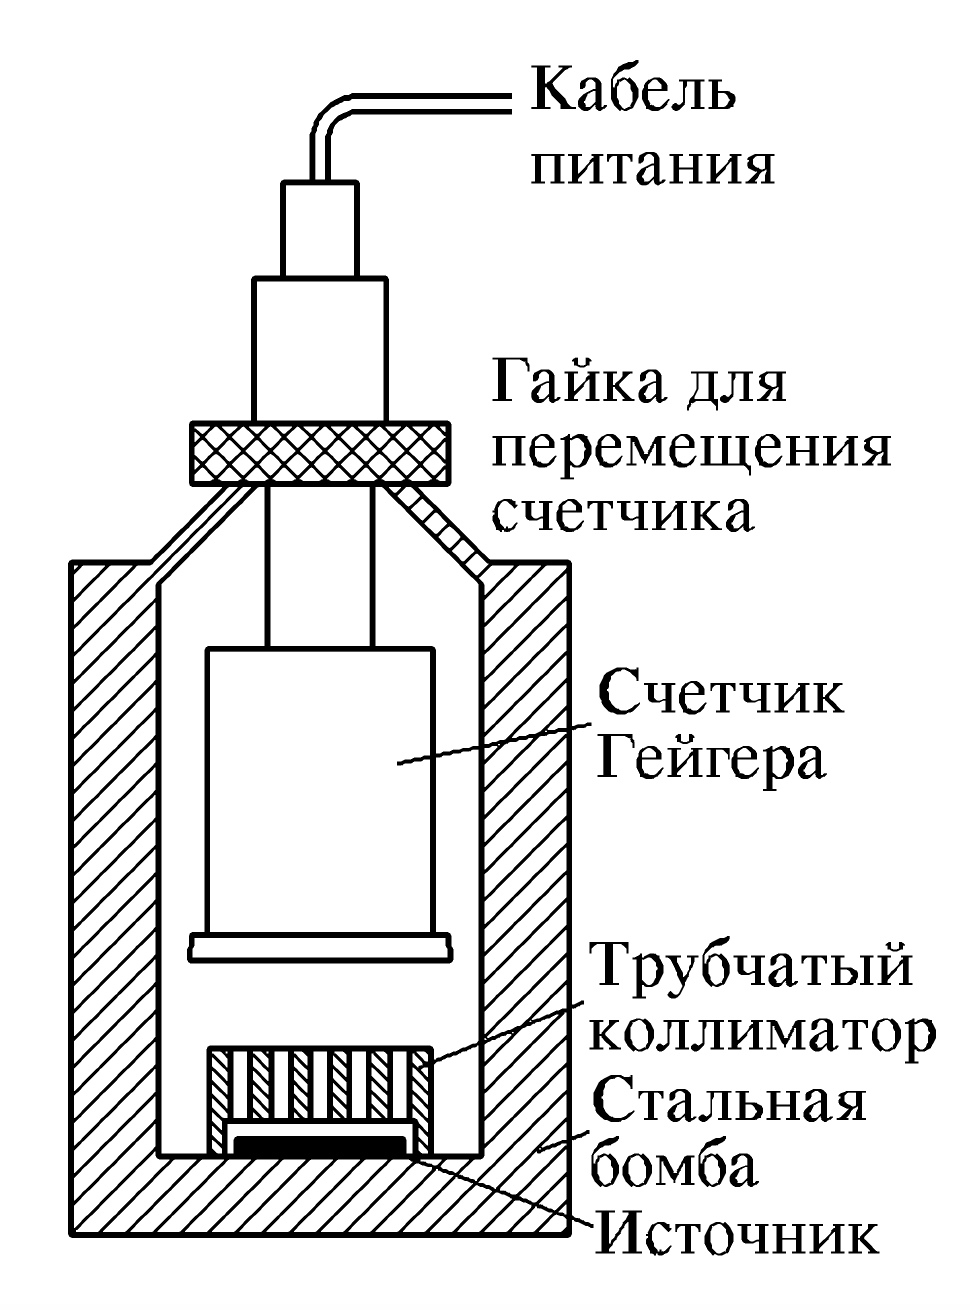
\includegraphics[width=\linewidth]{Geyger}
		\caption{Схема торцевого счетчика Гейгера}
		\label{ris geyger}
	\end{wrapfigure}
	
	Для определения пробега альфа-частиц с помощью счетчика радиоактивный источник помещается на дно стальной цилиндрической бомбы
	(рис. \ref{ris geyger}), в которой может перемещаться торцевой счетчик Гейгера. Его
	чувствительный объем отделен от наружной среды тонким слюдяным
	окошком, сквозь которое могут проходить альфа-частицы. Рабочее напря-
	жение счетчика указано на установке.
	
	Импульсы, возникающие в счетчике, усиливаются и регистрируются пересчетной схемой. Путь частиц в воздухе зависит от расстояния между источником и счетчиком. Перемещение счетчика производится путем вращения гайки, находящейся на крышке бомбы. Расстояние
	между счетчиком и препаратом измеряется по шкале, нанесенной на
	держатель счетчика. Счетчик не может быть придвинут к препарату ближе чем на 10 мм, т. к. между источником и счетчиком установлен коллиматор, изготовленный из плотно сжатых металлических трубок. Отверстия трубок пропускают к счетчику только те альфа-частицы, которые вылетают из источника почти перпендикулярно его поверхности.
	
	\subsection{Ионизационная камера}
	
	Ионизационная камера --- прибор для количественного измерения
	ионизации, произведенной заряженными частицами при прохождении
	через газ. Камера представляет собой наполненный газом сосуд с двумя электродами (схема камеры приведена на рис. \ref{ris Ion}). Сферическая стенка прибора служит одним из электродов, второй электрод вводится в газ через изолирующую пробку. К электродам подводится постоянное напряжение от источника ЭДС.
	
	Заполняющий сосуд газ сам по себе не проводит электрический ток, возникает он только при прохождении быстрой заряженной частицы, которая рождает в газе на своем пути ионы.
	
	Поместим на торец внутреннего электрода источник
	ионизирующего излучения (в нашем случае это источник
	альфа-частиц $ ^{239}_{94} $Pu), заполним объем камеры воздухом и начнем
	постепенно увеличивать разность потенциалов между электродами. Ток, протекающий через камеру, вначале будет резко возрастать, а затем, начиная с некоторого напряжения $ V_0 $, станет постоянным, т. е. "<выйдет на плато">.  Предельный ток $ I_0 $ будет равен $ I_0 = n_0e $,
	где $ n_0 $ --- число пар ионов, образуемых в секунду в объеме камеры, а $ e $ --- заряд электрона.
	
	\begin{wrapfigure}[16]{l}{0.37\linewidth}
		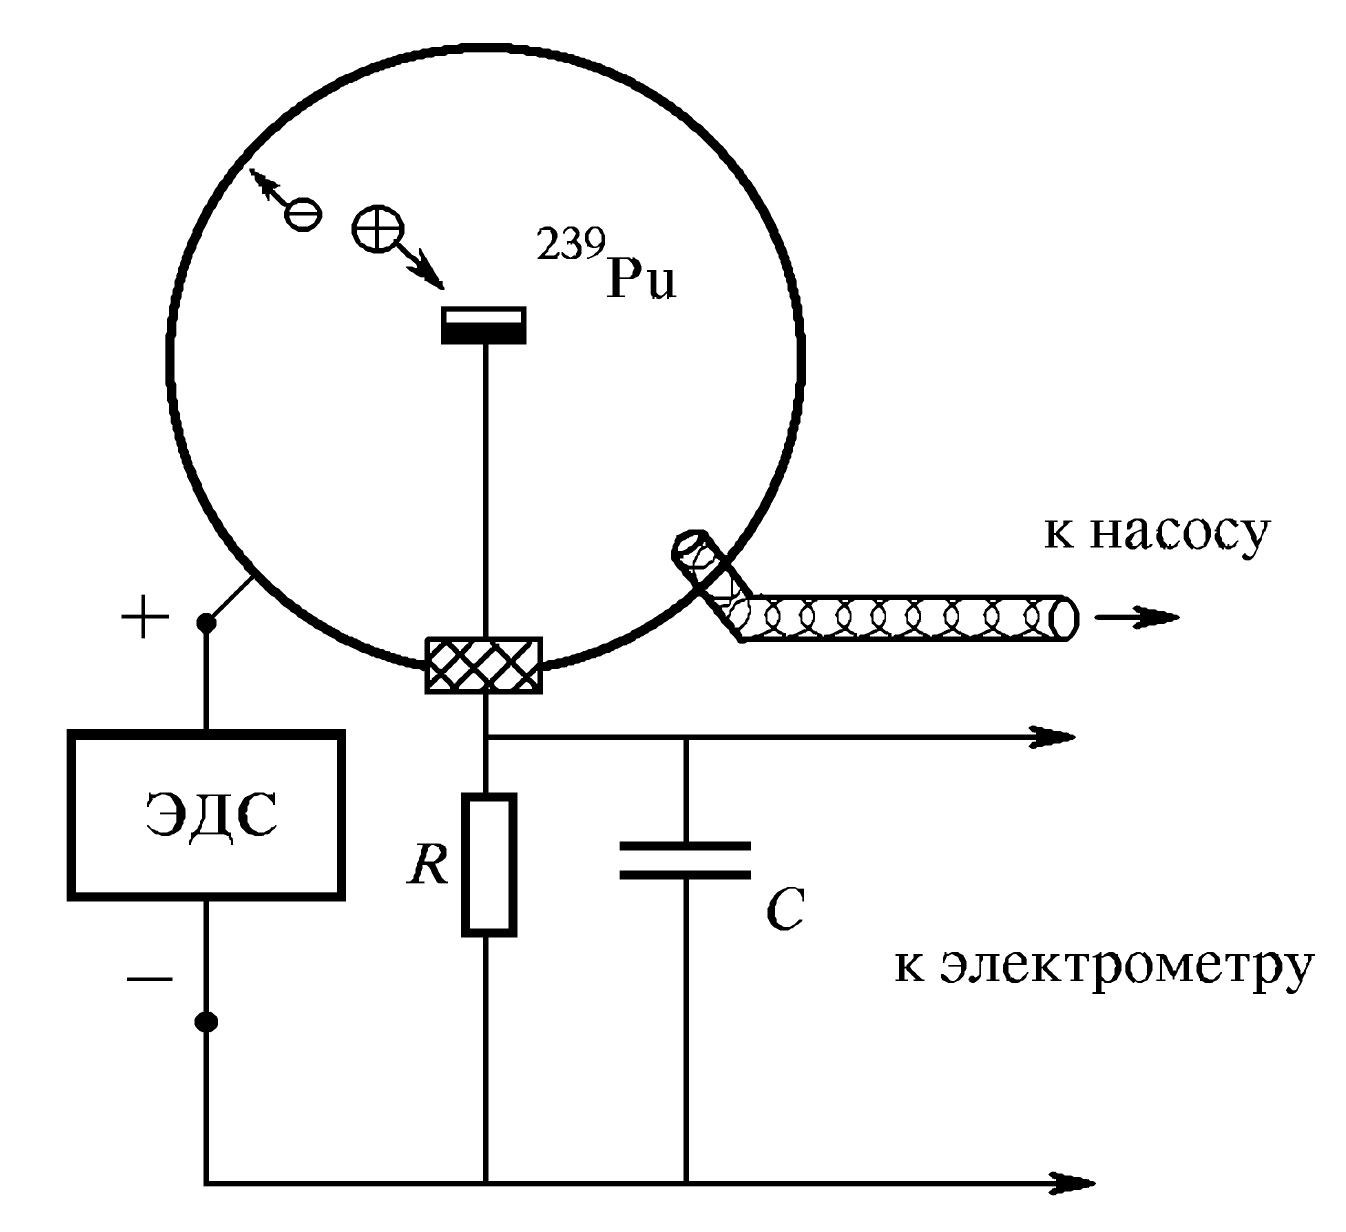
\includegraphics[width=\linewidth]{Ion}
		\caption{Схема устройства ионизационной камера}
		\label{ris Ion}
	\end{wrapfigure}
	
	Прохождение тока через камеру регистрируется посредством измерения напряжения на включенном в цепь камеры сопротивлении $ R $.
	Так как средняя энергия ионизации атомов воздуха составляет около 30 эВ, то альфа-частица с энергией 3 МэВ образует на своем пути около $ 10^5 $ электронов, им соответствует заряд $1,6 \x 10^{-14} $ Кл. Чтобы
	столь малое количество заряда, создаваемое проходящей через камеру одной альфа-частицей, вызывало измеряемое напряжение, емкость $ C $
	должна быть мала.
	
	Так как подвижность электронов примерно в 1000 раз больше подвижности ионов, то подбором параметров $ RC $-цепочки можно выделить импульсы тока, соответствующие только возникающей электронной компоненте. Реально регистрация электронной компоненты
	импульса тока обеспечивается при величине постоянной времени $ RC $-
	цепочки в несколько микросекунд.
	Если число проходящих через камеру альфа-частиц достаточно велико, то можно регистрировать не заряд, а величину возникающего тока, которая, естественно, пропорциональна интенсивности альфа-частиц. В
	токовом режиме величину постоянной времени $ RC $-цепочки устанавливают равной нескольким секундам, а работающую в этом режиме
	камеру называют токовой.
	
	\begin{wrapfigure}[15]{r}{0.3\linewidth}
		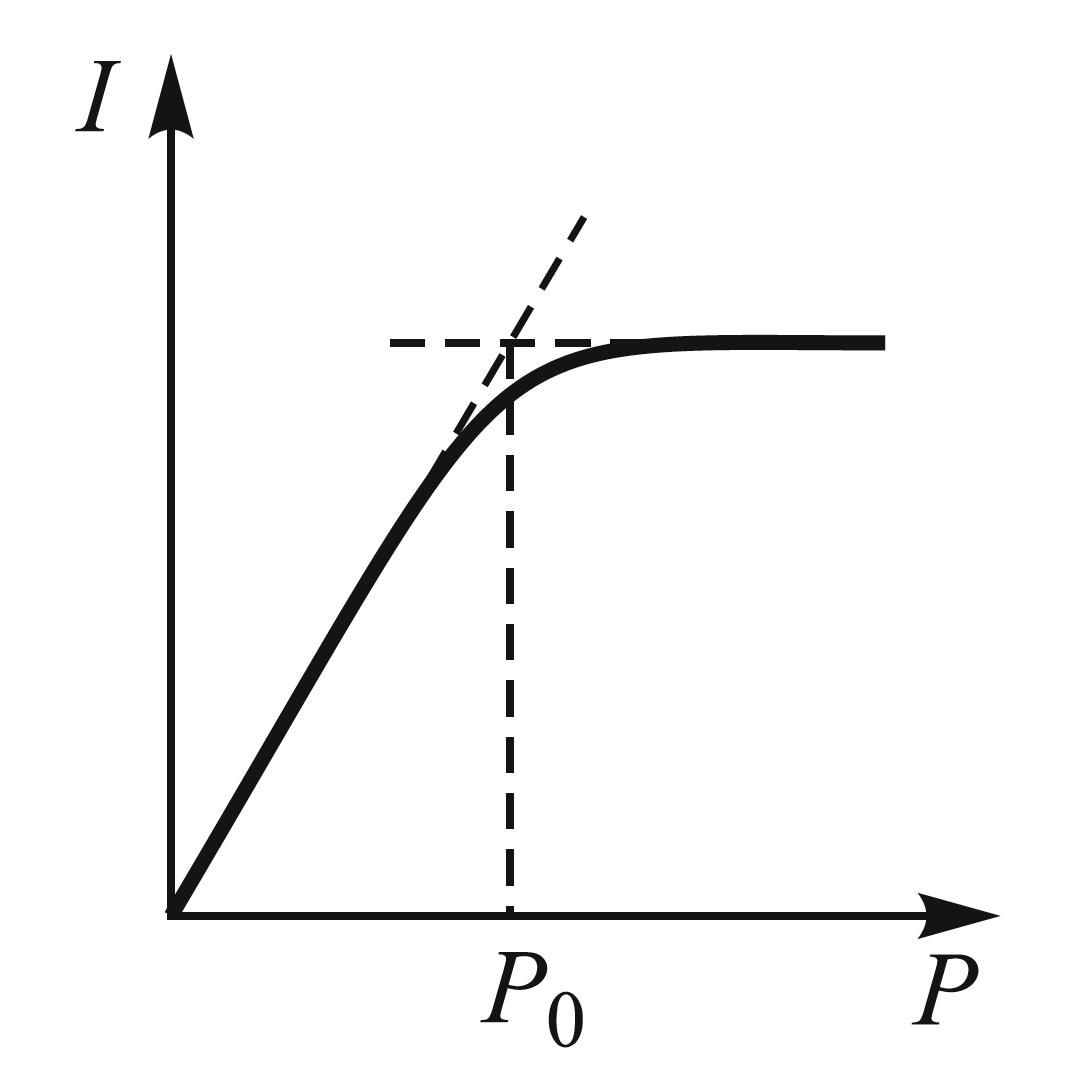
\includegraphics[width=\linewidth]{PotI}
		\caption{Характерная кривая зависимости
			тока ионизационной камеры от давления.
			Ионизация создается $ \alpha $-частицами}
		\label{ris PotI}
	\end{wrapfigure}
	
	При изменении давления в камере ионизационный ток меняется так, как это показано на рис. \ref{ris PotI}. При небольших давлениях газа
	альфа-частицы передают часть энергии стенкам камеры. По достижении
	давления $ P_0 $ все они заканчивают свой пробег внутри газа, и дальнейшее возрастание тока прекращается. Для определения давления $ P_0 $ чаще всего пользуются методом экстраполяции (полученная таким методом величина называется экстраполированным пробегом), продолжая наклонный и горизонтальный участки кривой до пересечения. Найденный таким образом пробег затем должен быть приведен к нормальному давлению и температуре $ 15 ^\circ C $.
	
	В данной работе измерение пробега альфа-частицы проводится по величине тока ионизации в сферической камере. Внутренним электродом
	камеры служит диск диаметром 5 мм, на который нанесен тонкий слой $ ^{239}_{94} $Pu, покрытый сверху тонкой защитной пленкой. Вторым электродом служит внешняя оболочка камеры --- полый шар с внутренним
	диаметром 100 мм. Оба электрода тщательно изолированы один от
	другого и от земли. Разность потенциалов между электродами составляет 300 В. Вакуумная установка содержит кран и манометр. Она позволяет изменять давление в камере от атмосферного до 10 мм рт. ст.
	Величина тока ионизации измеряется электрометром, состоящим из
	нескольких стандартных микросхем, по величине падения напряжения
	на сопротивлении $ R $ = 100 МОм ($ C = 10^{-8} $ Фарад, так что $ RC $ = 1 с).
	Значение измеряемого ионизационного тока (в пикоамперах) высвечивается на цифровом табло.
	
	
	
	
%	\section{Экспериментальная установка}
	
	\section{Выполнение работы}
	
		\subsection{Счетчик Гейгера}
		
		Включим счетчик Гейгера и дадим ему прогреться в течении 10 минут. Убедимся, что он регистрирует альфа-частицы. Затем проведем измерения зависимости скорости счета частиц $ N $ от расстояния между источником и счетчиком $ l $, начиная с минимально допустимых 10 мм и до 40мм (по факту, уже после $ l \gtrsim 25 $ мм остается только фон).
		
		Методика измерения счета и его погрешности стандартные: мы считаем число $ N' $ зарегистрированных частиц со статистической погрешностью $ \sigma_{N'}  = \sqrt{N'} $ и время регистрации $ t $, откуда получаем скорость счета $ N = N'/t $ и ее погрешность 
		
		 \begin{equation}\label{}
		\sigma_{N} = N \x \dfrac{\sqrt{N'}}{N'} = \dfrac{\sqrt{N'}}{t}
		\end{equation}
	
		Погрешность для $ l $ оценим как $ \sigma_l = 0,5 $ мм --- погрешность цены деления. Результаты измерений величин и их погрешностей занесем в таблицу и построим график.
		
			\begin{table}[H]
			\caption{Зависимость скорости счета частиц от расстояния между источником и счетчиком}
			\begin{center}
				\begin{tabular}{|c|c|c|c|c|c|}
					\hline 
					№ & $ l $, см & $ N $ & $ t $, с & $ N', \; с^{-1} $ & $ \sigma_{N'}, \; с^{-1} $  \\ 
					\hline 
				1 & 10 & 1104 & 74.9 & 14.74 & 0.44 \\
				2 & 13 & 1167 & 75.1 & 15.54 & 0.45 \\
				3 & 15 & 1175 & 75 & 15.67 & 0.46 \\
				4 & 16 & 1146 & 74.9 & 15.3 & 0.45 \\
				5 & 17 & 659 & 74.7 & 8.82 & 0.34 \\
				6 & 18 & 134 & 75 & 1.79 & 0.15 \\
				7 & 19 & 39 & 74.9 & 0.52 & 0.08 \\
				8 & 20 & 34 & 74.3 & 0.46 & 0.08 \\
				9 & 22 & 18 & 74.9 & 0.24 & 0.06 \\
				10 & 25 & 19 & 75.2 & 0.25 & 0.06 \\
				11 & 30 & 12 & 74.7 & 0.16 & 0.05 \\
				12 & 35 & 14 & 74.7 & 0.19 & 0.05 \\
				13 & 40 & 13 & 74.9 & 0.17 & 0.05 \\
					\hline 
				\end{tabular} 
			\end{center}
			\label{table g}
		\end{table}
	
	Профитируем линейный участок при $ l \in [16,19] $ мм. Результаты фита сведем в таблицу.
		
		\begin{figure}[h!]
			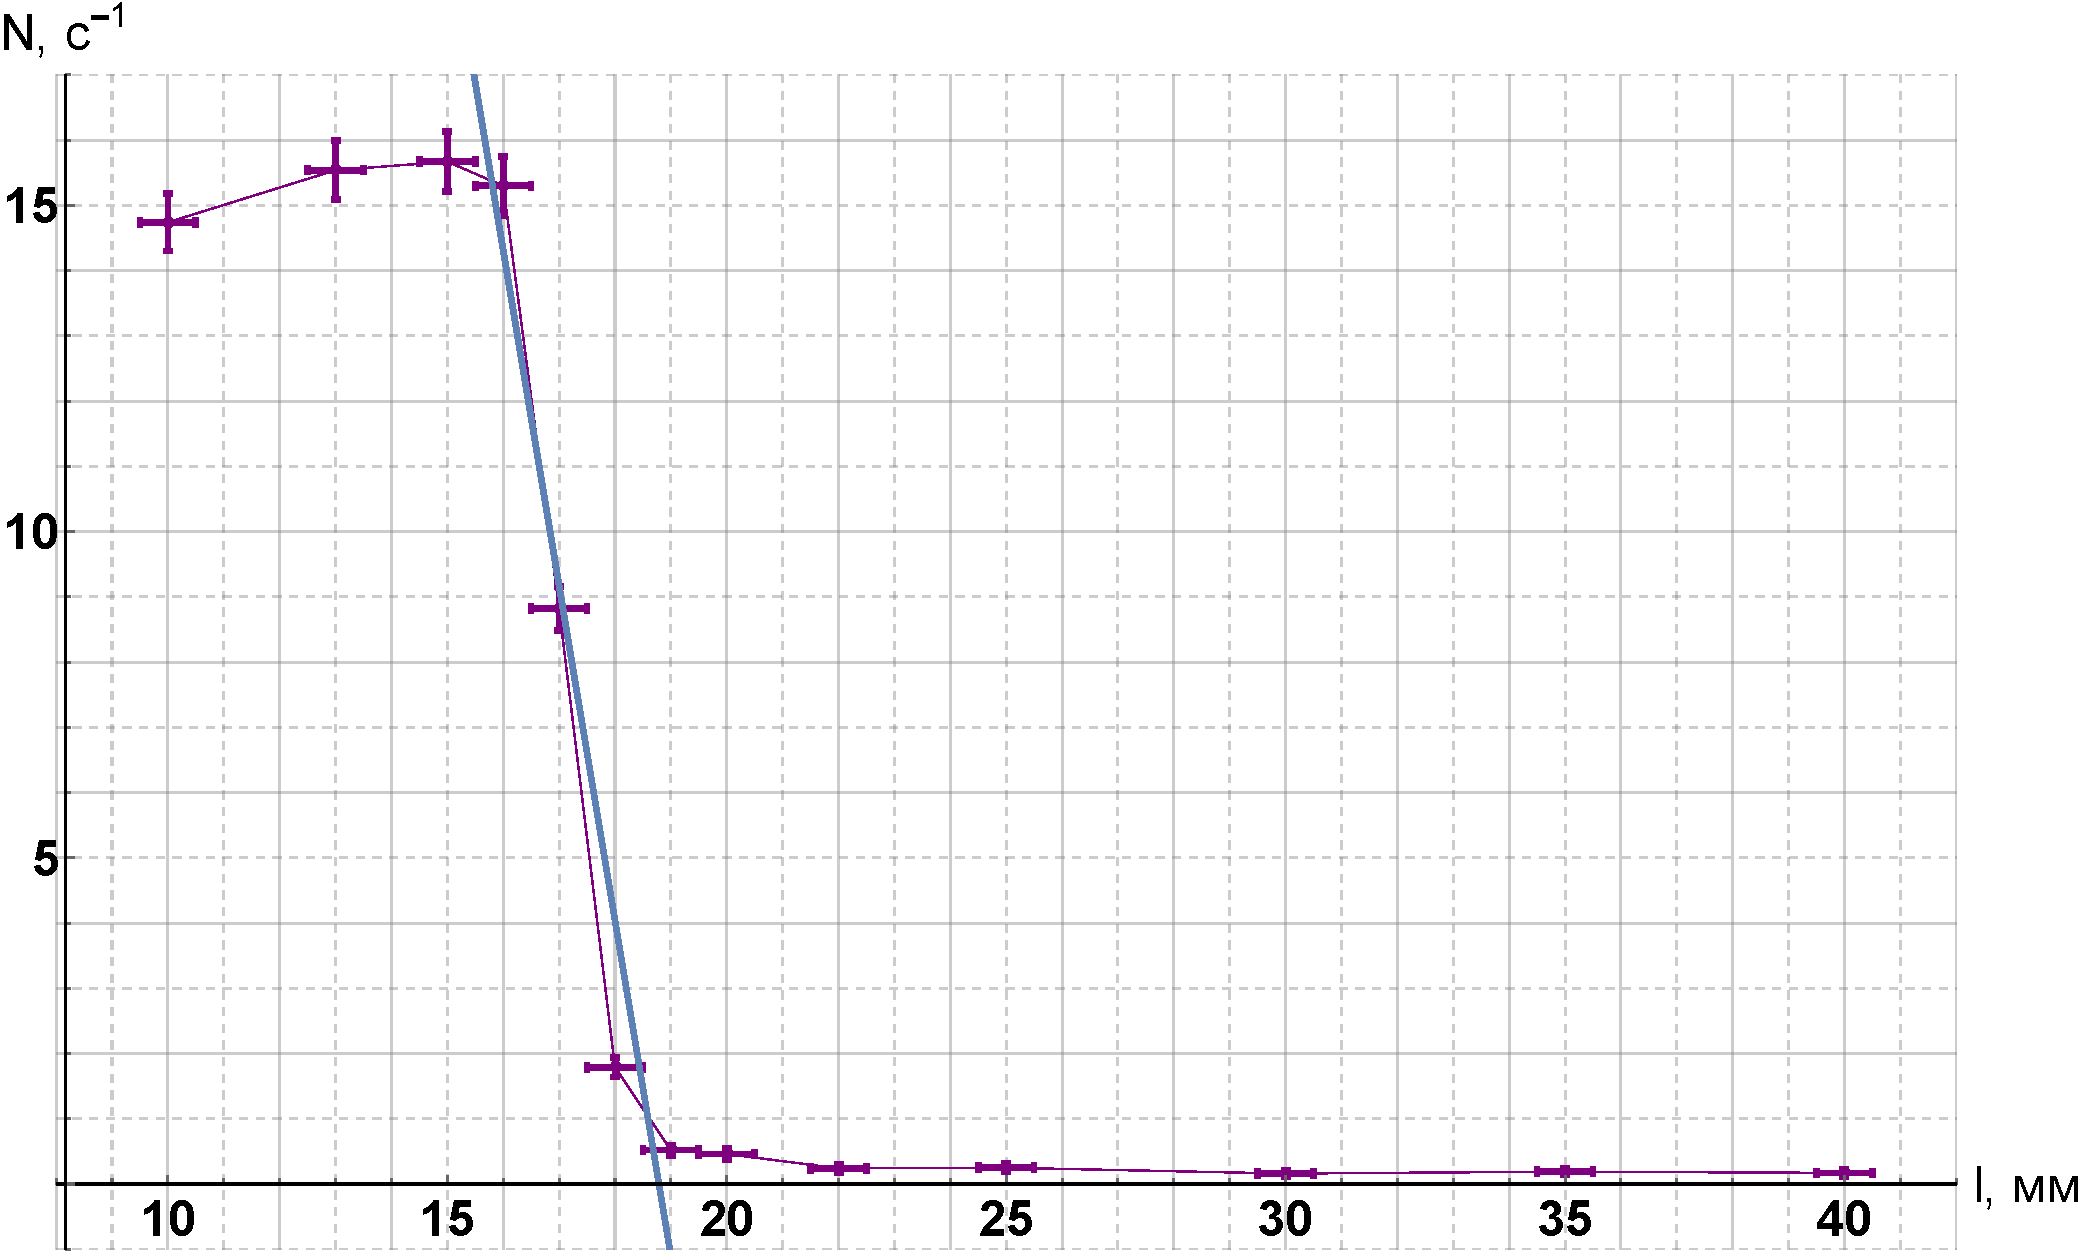
\includegraphics[scale=0.5]{graf_g.pdf}
			\caption{Зависимость скорости счета частиц от расстояния между источником и счетчиком}
			\label{graf_g}
		\end{figure} 
	
		\begin{table}[H]
			\caption{Фит рис. \ref{graf_g} функцией $ y = ax + b $}
			\begin{center}
				\begin{tabular}{|c|c|c|}
					\hline
					& \text{Estimate} & \text{Standard Error} \\
					\hline
					 b & 96,3 & 10,4 \\
					a & -5.14 & 0.34 \\
					\hline 
				\end{tabular} 
			\end{center}
			\label{}
		\end{table}
		
		 Экстраполируем полученую прямую до пересечения с осью абсцисс. Отсюда получаем экстраполированную длину пробега
		 
		 \begin{equation}\label{}
		 R_э = \dfrac{b}{a} \approx 18,9 \pm 1,9 \; мм \te R'_э = \rho R_э = (2,44 \pm 0,24)\x 10^{-3} \; г/см^2
		 \end{equation}
		
		Среднюю длину пробега оценим как $ R_{ср} \backsimeq 17,5 \pm 1,5 $ мм $ \te R'_ср = \rho R_ср = (2,26 \pm 0,19)-x^{-3} \; г/см^2 $
		
		Энергию таких альфа-частицы можно оценить по эмпирической формуле 
		
		\begin{equation}\label{}
		R = 0,32 E^{3/2} \te E_э = \approx 3,26 \pm 0,22 \; МэВ, \quad E_{ср} = \approx 3,10 \pm 0,18 \; МэВ
		\end{equation}
		
		\subsection{Ионизационная камера}
		
		Включив питание установки, измерим при атмосферном давлении $ P_а = 102,6 $ кПа = 769,9~Торр (измеренном барометром) ток $ I_а = 820 $ пА. Температура $ T = 298 $ К. После этого откачаем воздух из камеры до давления порядка $ \backsimeq 10 $ Торр и снимем зависимость тока от давления.
		
		Погрешность давления оценим как цену деления --- $ \sigma_P = 5 $ Торр, погрешность $ \sigma_I = 3 $ пФ. Результаты измерения занесем в таблицу и построим график.
		
			\begin{table}[h!]
			\caption{Зависимость тока от давления}
			\begin{center}
				\begin{tabular}{|c|c|c|}
					\hline 
					№ & $ P $, Торр & $ I, $ пА  \\ 
					\hline 
				1 & 16 & 6 \\
				2 & 56 & 63 \\
				3 & 101 & 112 \\
				4 & 121 & 155 \\
				5 & 171 & 230 \\
				6 & 211 & 285 \\
				7 & 241 & 348 \\
				8 & 281 & 411 \\
				9 & 321 & 482 \\
				10 & 361 & 549 \\
				11 & 416 & 658 \\
				12 & 471 & 760 \\
				13 & 491 & 792 \\
				14 & 511 & 822 \\
				15 & 516 & 823 \\
				16 & 536 & 850 \\
				17 & 546 & 862 \\
				18 & 561 & 859 \\
				19 & 581 & 858 \\
				20 & 601 & 859 \\
				21 & 611 & 861 \\
				22 & 631 & 854 \\
				23 & 641 & 860 \\
				24 & 651 & 857 \\
				25 & 671 & 860 \\
					\hline 
				\end{tabular} 
			\end{center}
			\label{table ion}
		\end{table}
	
	
		\begin{figure}[h!]
		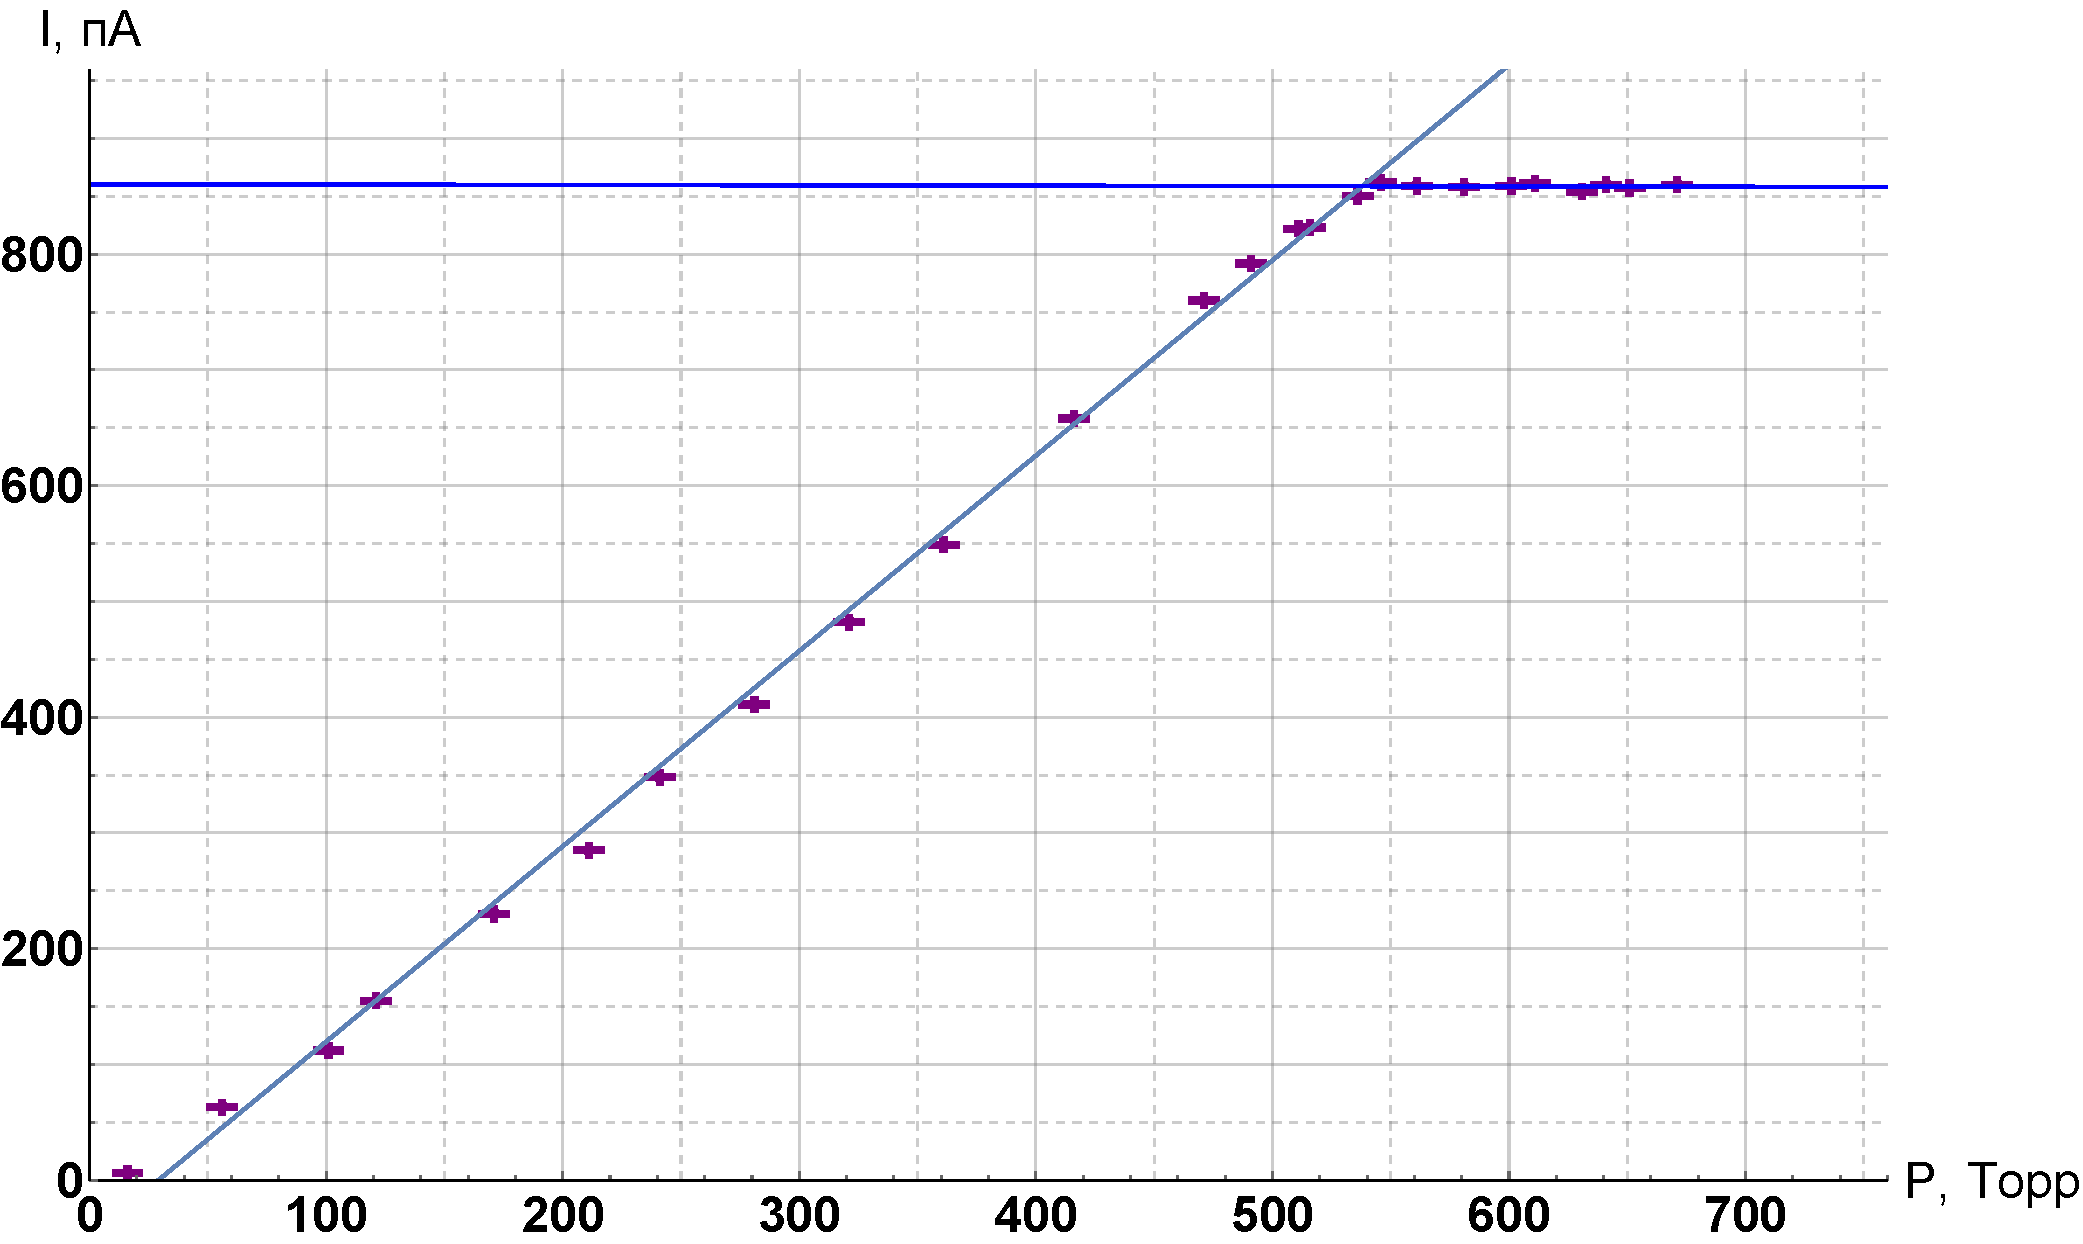
\includegraphics[scale=0.5]{graf_ion.pdf}
		\caption{Зависимость тока от давления в ионизационной камере}
				\label{graf_ion}
	\end{figure} 

	Построим две прямых, соответствующих линейным участкам графика. Результаты фита сведем в таблицу: 
	
	\begin{table}[H]
		\caption{Фит рис. \ref{graf_ion} функцией $ y = ax + b $} %TODO
		\begin{center}
			\begin{tabular}{|c|c|c|}
				\hline
				Участок графика (по оси х) & $ a $ & $ b $ \\
				\hline
				 $ x \in [0, 511] $& $ 1,69 \pm 0,03 $  & $ -49 \pm 8 $ \\
				  $ x \in [561, 671] $ & $ 0,00 \pm 0,02 $ & $ 860 \pm 15  $\\
				\hline 
			\end{tabular} 
		\end{center}
		\label{compt_fit}
	\end{table}
	
	Их пересечение дает нам значение 
	
	\begin{equation}\label{}
	P_0 = \dfrac{b_2 - b_1}{a_1 - a_2} \approx (538 \pm 21) \; Торр 
	\end{equation}
	
	Так как пробег $ R_l = 5 $ см задается размером камеры, приведем его к н.у.:
	
	\begin{equation}\label{}
	R_э = R_l \dfrac{\rho}{\rho_0} = R_l \dfrac{PT_0}{P_0T} \approx (3,41 \pm 0,13) \; см \te R'_э \approx (4,40 \pm 0,18)\x 10^{-3} \; г/см^2
	\end{equation}
	
	Энергию такой альфа-частицы можно оценить по эмпирической формуле 
	
	\begin{equation}\label{}
	R = 0,32 E^{3/2} \te E_э = \left(  \dfrac{R_э}{0,32} \right)^2/3 \approx 4,84 \pm 0,09 \; МэВ
	\end{equation}
	
	\section{Вывод}
	
	В работе был измерен пробег альфа-частиц от $ ^{239}  $Pu двумя способами :с помощью торцевого счетчика Гейгера и ионизационной камеры. По полученным данным была определена энергия альфа - частиц.

	
	При работе с ионизационной камерой пробег и энергия получились близкими к ожидаемым (из таблиц при $ E = 5 $ МэВ получаем $ R = 3,29 $ см для воздуха). При работе со счетчиком Гейгера значения пробега и энергий ниже табличных. Это можно объяснить тем, что часть энергии альфа-частиц тратится на прохождение слюдяной пластинки, прикрывающей счетчик, и пленки, закрывающей источник. 
	
	Если плотность бумаги равна $ 1,2 \; г/см^3 $, следовательно, лист бумаги толщины $~l~\geq~R'/\rho \hm{=}36, 6 $~мкм не пропустит альфа-частицы от $ ^{239}  $Pu.
\end{document}
